\section{Пример}

%------------------------------------------------

\begin{frame}
	\frametitle{Обычный текст}
    Обычный текст пишется так

    \textbf{Вот так}

    \Huge 

    И даже так

    \tiny может и вот так

    \normalsize
    И в конце концов снова так
\end{frame}

%------------------------------------------------

\begin{frame}
	\frametitle{Списки}
    \begin{enumerate}
        \item Один
        \item Два
    \end{enumerate}

    \begin{itemize}
        \item Один
        \item Два
    \end{itemize}
\end{frame}

%------------------------------------------------

\begin{frame}[fragile]
	\frametitle{Код}
    не забудь [fragile]
    коменты не работают
\begin{cpp}
cout << "Python is bad\n";
\end{cpp}
	
\end{frame}

%------------------------------------------------

\begin{frame}
	\frametitle{Картинки}
    \center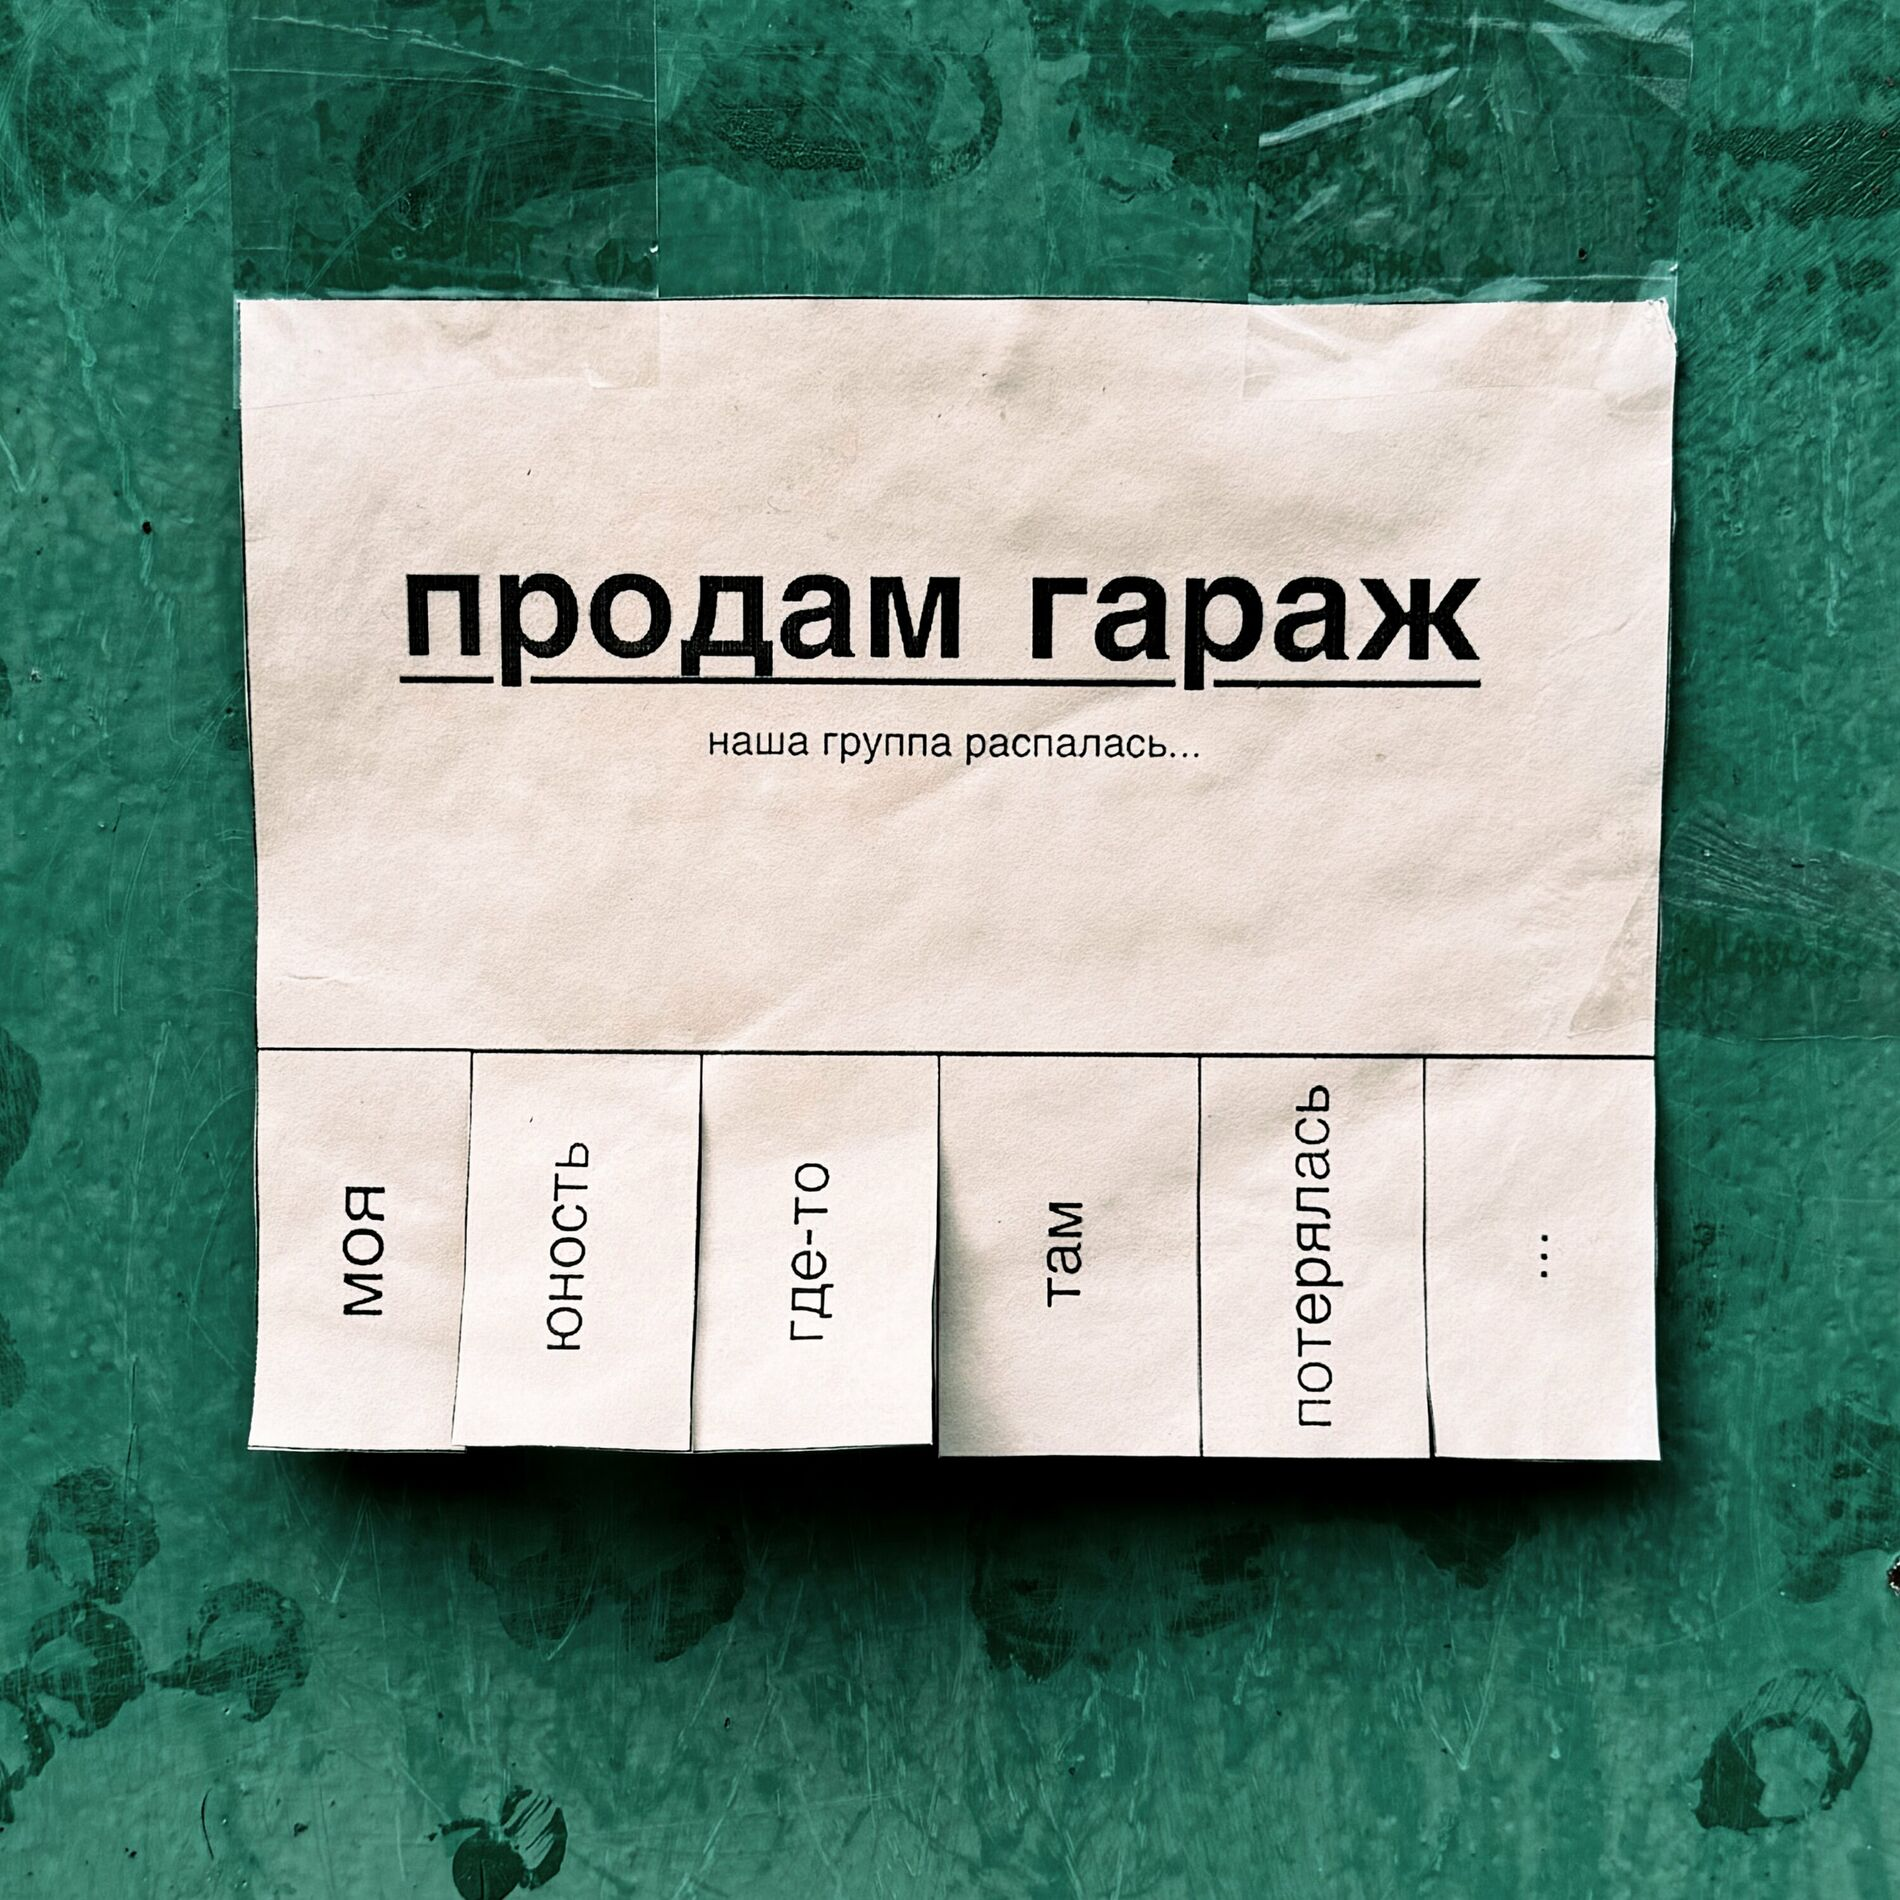
\includegraphics[scale=0.4]{image.jpg}

\end{frame}

%------------------------------------------------

\begin{frame}
	\frametitle{Графики}
	
    \begin{tikzpicture}
        \begin{axis}[
            xmin=0, xmax=100,
            ymin=0, ymax=20,
            xtick={0,100},
            ytick={0,120},
            legend pos=north east,
            ]

            \addplot[
                color=blue,
                mark=none,
                samples=200,
                domain=0:100,
                unbounded coords=jump
                ]
                {sqrt(x)};

            \addplot[
                color=red,
                mark=none,
                samples=200,
                domain=0:100,
                unbounded coords=jump
                ]
                {x};

            \legend{$\sqrt(x)$, 
                    $x$}
        \end{axis}
    \end{tikzpicture}
\end{frame}
